Pour chacune des affirmations suivantes, indiquer si elle est vraie ou fausse en justifiant votre choix.

Une réponse non justifiée ne sera pas prise en compte dans l'évaluation.

Les quatre questions sont indépendantes.

\begin{enumerate}
	\item On considère la fonction $f$ définie sur $\R$ par
	\[f(x)=\left(-\dfrac{1}{2} x+3\right)^{5}\]

	\textbf{Affirmation 1 :} La fonction $f$ est convexe sur $\R$.

	\item Une urne contient 32 jetons numérotés de 1 à 32 indiscernables au toucher.

	On tire simultanément 5 jetons de cette urne.

	On appelle tirage la liste non ordonnée des numéros des cinq jetons tirés.

	\textbf{Affirmation 2 :} Le nombre de tirages possibles contenant au moins un multiple de 8 est égal à \np{103096}.

	\item On considère l'arbre de probabilités ci-dessous.

	\begin{center}
	\begin{tikzpicture}[xscale=1,yscale=1.2,baseline={(R.base)}]
		
		\tikzstyle{noeud}=[fill=white,circle,inner sep=2pt]
		\tikzstyle{feuille}=[fill=white,circle,inner sep=2pt]
		\tikzstyle{etiquette}=[pos=0.6,fill=white, inner xsep=3pt, inner ysep=1.5pt]
		
		\def\DistanceInterNiveaux{3}
		\def\DistanceInterFeuilles{0.8}
		
		\def\NiveauA{(0)*\DistanceInterNiveaux}
		\def\NiveauB{(1)*\DistanceInterNiveaux}
		\def\NiveauC{(2)*\DistanceInterNiveaux}
		\def\InterFeuilles{(-1)*\DistanceInterFeuilles}
		
		\node[noeud] (R) at ({\NiveauA},{(1.5)*\InterFeuilles}) {};
		\node[noeud] (Ra) at ({\NiveauB},{(0.5)*\InterFeuilles}) {$A$};
		\node[feuille] (Raa) at ({\NiveauC},{(0)*\InterFeuilles}) {$B$};
		\node[feuille] (Rab) at ({\NiveauC},{(1)*\InterFeuilles}) {$\overline{B}$};
		\node[noeud] (Rb) at ({\NiveauB},{(2.5)*\InterFeuilles}) {$\overline{A}$};
		\node[feuille] (Rba) at ({\NiveauC},{(2)*\InterFeuilles}) {$B$};
		\node[feuille] (Rbb) at ({\NiveauC},{(3)*\InterFeuilles}) {$\overline{B}$};
		
		\draw (R.east)--(Ra.west) node[etiquette] {$\dfrac{2}{5}$};
		\draw (Ra.east)--(Raa.west) node[etiquette] {$\dfrac{1}{4}$};
		\draw (Ra.east)--(Rab.west);
		\draw (R.east)--(Rb.west);
		\draw (Rb.east)--(Rba.west);
		\draw (Rb.east)--(Rbb.west) node[etiquette] {$\dfrac{7}{10}$};
	\end{tikzpicture}
	\end{center}

	\textbf{Affirmation 3:} \quad $P_{B}\big(\,\overline{A}\,\big)=\dfrac{9}{50}$.

	\item On considère l'équation différentielle
	\[(E): \quad y'+y=\e^{-x} \cos (x),\]
	où $y$ est une fonction de la variable $x$, dérivable sur $\R$.

	\textbf{Affirmation 4 :} La fonction $h$ définie sur $\R$ par $h(x)=\e^{-x} \sin (x)$ est solution de $(E)$ sur $\R$.

	\textbf{Affirmation 5 :} Les solutions de $(E)$ sur $\R$ sont les fonctions $k$ définies sur $\R$ par
	\[k(x)=C \e^{-x} \sin (x) \quad\text { où } C \text { est une constante réelle. }\]
\end{enumerate}
